\documentclass[a4paper]{article}
\usepackage{color}
\usepackage{listings}
\usepackage{tcolorbox}
\usepackage[utf8]{inputenc}
\usepackage{graphicx}
\usepackage{tabto}
\usepackage{float}
\usepackage{amsmath}
\usepackage{amssymb}
\usepackage{amsthm}
\usepackage{algorithm}
\usepackage{algpseudocode}
\usepackage{siunitx}
\usepackage{hyperref}
\usepackage{array}
\usepackage{MnSymbol,wasysym}
\usepackage{multirow}
\usepackage{caption}
\usepackage{subcaption}
\usepackage[english]{babel}
\newtheorem{theorem}{Theorem}[section]
\newtheorem{corollary}{Corollary}[theorem]
\newtheorem{lemma}[theorem]{Lemma}
\theoremstyle{definition}
\newtheorem{definition}{Definition}[section]
\theoremstyle{remark}
\newtheorem{remark}{Remark}[section]
\newtheorem{example}{Example}[section]
\usepackage{geometry}
 \geometry{
 a4paper,
 total={150mm,254mm},
 left=30mm,
 top=20mm,
 }
 \newcommand{\heart}{\ensuremath\heartsuit}
\newcommand{\butt}{\rotatebox[origin=c]{180}{\heart}}
\lstset{language=C++,
keywordstyle=\color{blue},
stringstyle=\color{red},
commentstyle=\color{green},
morecomment=[l][\color{magenta}]{\#}
}

\title{Assignment \#2}
\author{Michał Przybylski, Francesco Ragaini}
\date{February 2025}
\begin{document}
\maketitle
\section*{Task 1}
\tab 
In order to build an algorithm that is working for the master-worker problem we need to figure out the 
two functions worker and master. They are builted in that way\\
\begin{minipage}{0.45\textwidth}
\begin{algorithm}[H]
\caption{Master Algorithm version 0}
\begin{algorithmic}[1]
\State Initialize all the needed variables: \texttt{sent} $\gets$ 0, \texttt{done} $\gets$ 0, \texttt{workdone} $\gets$ 0
\For{each worker}
    \State Send a task to the worker
    \State \texttt{sent} $\gets$ \texttt{sent} + 1
\EndFor
\While{\texttt{sent} $<$ \texttt{total\_task}}
    \State receive a task done (blocking)
    \State send a new task (\texttt{task\_to\_do[sent]}) to the same worker (blocking)
    \State \texttt{result[done]} $\gets$ \texttt{worker}
    \State \texttt{done}++
    \State \texttt{sent}++
\EndWhile
\For{each worker}
    \State receive a task done (blocking)
    \State sent the sleeping message to the same worker (blocking)
    \State \texttt{result[done]} $\gets$ \texttt{worker}
    \State \texttt{done}++
\EndFor
\end{algorithmic}
\end{algorithm}
\end{minipage}
\hfill
\begin{minipage}{0.45\textwidth}
\begin{algorithm}[H]
\caption{Worker Algorithm version 0}
\begin{algorithmic}[1]
\While{true}
    \State receive a task from the master (blocking)
    \If{task is sleeping message}
        \State break
    \EndIf
    \State perform the task
    \State send the result to the master (blocking)
\EndWhile
\end{algorithmic}
\end{algorithm}
\end{minipage}\\
After this algorithm, the master is able to perform statistics on the time needed for the program.\\
After that, we tried to improve the performance of the program, leading to version 1, 
which introduces some non-blocking commands. In particular, the first sending is non-blocking, 
the send inside the while loop is also non-blocking (the check for it is after the operations in the while loop), 
and the send inside the last for loop is non-blocking (and they are checked at the end of the master function).\\
We now tried to improve the algorithm once more, and the changes are: the first task is sent before the others 
(the idea is to make the first worker finish its tasks at different times than the others in order to reduce the queue at 
the master's door). The send inside the while loop is not checked (in fact, this program is really fast and reliable, 
so it is not really necessary to check all the sends). It is not possible to make the receive inside the while loop non-blocking 
because we need the master to wait for the workers to complete the tasks.\\
(IT MIGHT BE A GOOD IDEA TO SHOW THE UPDATED ALGORITHM HERE, BUT I DON'T THINK THERE'S ENOUGH SPACE).\\
We can now check the elapsed times to see if our improvements are making the code faster, this is 
done in figure \ref{fig:figure1}
\begin{figure}
    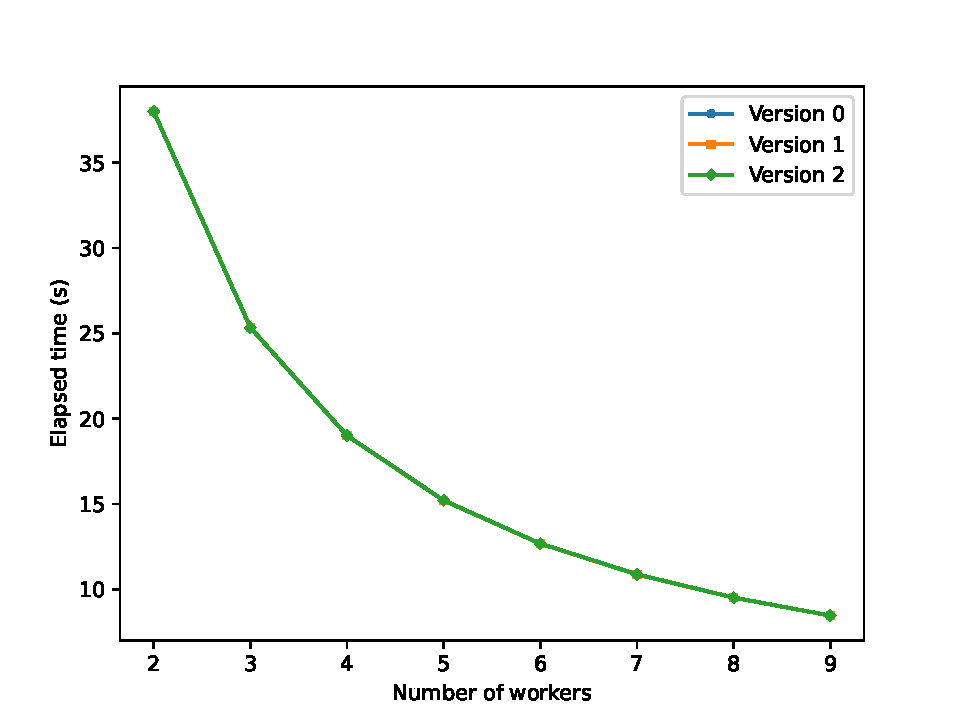
\includegraphics[width=\textwidth]{ex1.pdf}
    \label{fig:figure1}
\end{figure}

As is possible to see our changing are not really improving the times, but is also possible that those changing 
are significant just for high number of workers (in fact all the changing are ment to reduce the time that the worker need to wait 
at the master door and since they are just a few this time is already small.) but since this first task was just ment to 
set a benchmark we can bring this question with us for the next one.
\section*{Task 2}
We can finally mouve to the second question that is really more interesting in term of physical applications, in fact 
here the tasks are ment to be usefull.
We can now expose the algortihm for both master and worker that are similar to the version 0 of the first question.\\
\begin{minipage}{0.45\textwidth}
\begin{algorithm}[H]
\caption{Master Algorithm version 0}
\begin{algorithmic}[1]
\State Initialize all the needed variables: \texttt{done} $\gets$ 0, \texttt{sent} $\gets$ \texttt{nworker}
\State \texttt{settings\_sorted} $\gets$ \texttt{vector of size n\_settings}
\For{each worker $i$ from 1 to \texttt{nworker}}
    \State Send \texttt{settings[i-1]} to worker $i$
\EndFor
\While{\texttt{sent} $<$ \texttt{n\_settings}}
    \State Receive \texttt{worker} from any source
    \State Receive \texttt{accu} from \texttt{worker}
    \State Receive \texttt{momentaneus\_setting} from \texttt{worker}
    \State Send \texttt{settings[sent]} to \texttt{worker}
    \State \texttt{accuracy[done]} $\gets$ \texttt{accu}
    \State \texttt{settings\_sorted[done]} $\gets$ \texttt{momentaneus\_setting}
    \State \texttt{done}++
    \State \texttt{sent}++
\EndWhile
\For{each worker}
    \State Receive \texttt{worker} from any source
    \State Receive \texttt{accu} from \texttt{worker}
    \State Receive \texttt{momentaneus\_setting} from \texttt{worker}
    \State \texttt{settings\_sorted[done]} $\gets$ \texttt{momentaneus\_setting}
    \State \texttt{accuracy[done]} $\gets$ \texttt{accu}
    \State Send \texttt{rest\_signal} to \texttt{worker}
    \State \texttt{done}++
\EndFor
\end{algorithmic}
\end{algorithm}
\end{minipage}
\hfill
\begin{minipage}{0.45\textwidth}
\begin{algorithm}[H]
\caption{Worker Algorithm version 0}
\begin{algorithmic}[1]
\While{true}
    \State receive \texttt{setting} from the master (blocking)
    \If{\texttt{setting[0]} is -999}
        \State break
    \EndIf
    \State perform the task and compute \texttt{acc}
    \State send \texttt{rank} to the master (blocking)
    \State send \texttt{acc} to the master (blocking)
    \State send \texttt{setting} to the master (blocking)
\EndWhile
\end{algorithmic}
\end{algorithm}
\end{minipage}\\
In this case as been necessary to add 3 send condition for the worker, in fact it needs to comunicate the informations 
about his ranking, the results and the settings that is using (this last part is really important, in fact in order to find the best 
settings is crucial to know which resolution is connected to which settings).\\ Is now time to try to improuve the code, 
the first two versions (version 1 and version 2) are made following the same ideas as before. 
The fact that we need to use 3 sent seems to be the main problem of the code, so we try to condens all the 
informations, this is done by passing one vector (called result with len = 10, 8 for the settings, 1 for the rank and 1 for the result ),
in this way the number of comunication is reduced and the master can work on it, to order the result, after it sent the new task to the 
worker that in this way is not loosing time. 
After a small conversionation with the TA we find out a better way to do it, in fact is possible to use MPI\_Status, ranking and 
tag to pass all the information in one command, the code inside the while  is now so 
\begin{algorithm}[H]
    \begin{algorithmic}
        \While{\texttt{sent} $<$ \texttt{n\_settings}}
    \State Receive \texttt{result} from any source (blocking)
    \State \texttt{worker} $\gets$ \texttt{result[0]}
    \State Send \texttt{settings[sent]} to \texttt{worker} (non-blocking)
    \State \texttt{settings\_sorted[done]} $\gets$ \texttt{result[2:]}
    \State \texttt{accuracy[done]} $\gets$ \texttt{result[1]}
    \State \texttt{done}++
    \State \texttt{sent}++
\EndWhile
\end{algorithmic}
\end{algorithm}
(ALSO IN THIS CAS WE CAN THING TO SHOW THE ALL ALGORITHM)
We can now see the difference between the different versions of the code for the number of workers (\ref{fig:figure2}) 
and the sequential code
\begin{figure}
    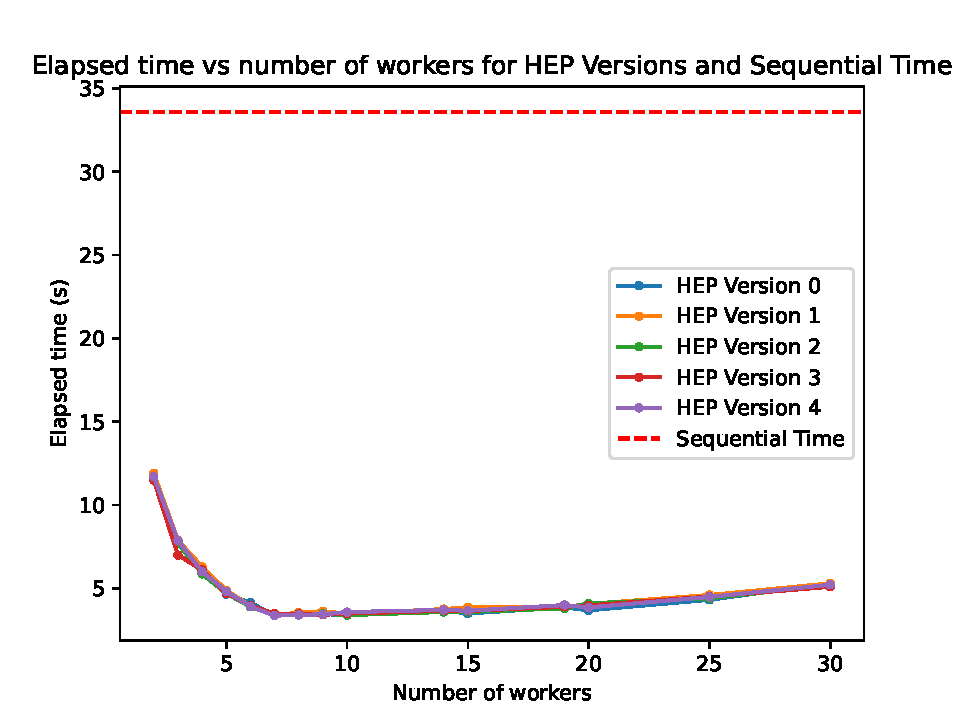
\includegraphics[width = \textwidth]{exercise2.pdf}
    \label{fig:figure2}
\end{figure}
To see better the behavior of it we can also look at the ratio between the version and the first version (see Figure \ref{fig:figure3}).
\begin{figure}
    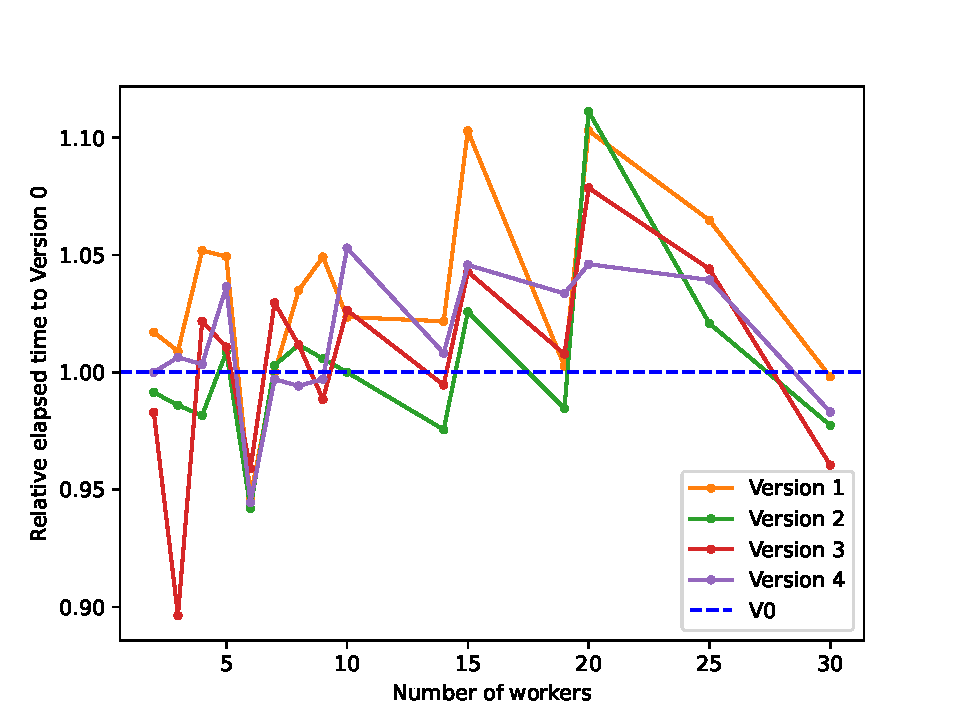
\includegraphics[width = \textwidth]{ex2.1.pdf}
    \label{fig:figure3}
\end{figure}
It is also important to underline that all the given results are checked to ensure that the final result 
(the best settings and its accuracy) 
is the same as the sequential one.\\
As is really clear from the plots, the different results are not reporting such a big difference, but we are sure that the last one 
is better for a higher number of workers, its behavior will be shown in Task 3. It is also important to notice that for some reason 
the time needed for a higher number of workers is increasing, this might be because the communication between the nodes 
is not as effective as we expected it to be. This will also be explored in Task 3. On the other hand the parallel code is working really 
faster that the sequential code.
\end{document}
